\chapter{Materials and Methods}
\label{ch:methods}

\section{Electrophysiology}
\label{sec:ephys}

\subsection{Subjects}

All experiments were conducted with Mongolian gerbils (Meriones unguiculatus). Gerbils were selected as an experimental animal for a number of reasons. First, gerbils were shown to have a good visual acuity (~ 1.75 cycles/deg grating acuity at 70 cd/m2; \cite{Baker1983}) and visual alertness (\cite{Ingle1981}). Second, gerbils are more active in the light part of the day cycle (\cite{Naumov1975}), suitable for experimental recordings. Finally, gerbils show better exploration of novel contexts and less dependency on moving along the boundaries (thigmotaxis) (\cite{STUERMER2003249}), which is highly important to reach high levels of arena occupancy across all experimental conditions.

In total, 9 wild-type animals from the local breeding facility were used. Among those, all 9 were used in the shift experiment, and 4 were recorded in the gain experiments, so some animals took part in both experimental paradigms. After the implantation of microelectrodes, animals were housed individually with a maintenance of the 12 hours light/dark cycle. A few days after the surgery and before the start of the experiments animals had ad libitum access to food and water. During the recordings, animals were kept on a food diet to maintain 90-95\% of their original ad libitum weight to increase the interest in random foraging for food pellets during the recording. All experiments were approved according to national and European guidelines on animal welfare (Reg. von Oberbayern, license number AZ 55.2-1-54-2532-70-2016).


\section{Implant design}
\label{sec:implant_design}

In the beginning, we used 4- or 8-tetrode Axona microdrives (Axona Ltd., U.K. http://www.axona.com/) to record from the dorsal CA1 region of the hippocampus. Later in the project, aimed at increasing the density of the recording sites in the brain area of interest as well as to have a possibility to reuse recording devices we chose the 64-channel Buzsaki H64 silicon probe as a candidate for electrophysiological recordings. In order to support implantation, maintenance and successful recovery of the probe after the end of the experiment, a set of custom components was designed. These include the microdrive, the base plate, the protecting box and a set of components supporting the implantation procedure.

\subsection{Microdrive}

The industrial microdrives (e.g. nano-Drives from Cambridge NeuroTech) are usually very expensive and do not allow reusing the recording device. The recent advances in 3D-printing allowed for custom design of the small components, necessary to build reliable microdrives within a short period of time. To be able to change to the procedure to using silicon probes instead of tetrode drives I designed a custom microdrive that meet the following characteristics:

\begin{itemize}
    \item the bottom size of the microdrive should not exceed 20 $mm^2$ to be able to be cemented on the gerbil skull, as well as the body of the microdrive should be fully contained inside the protecting box
    \item the weight of the microdrive should not exceed 2g to be able to carry by small animals
    \item the smallest stable movement of the shuttle of the microdrive should be in the range of 30 to 50 um
    \item the microdrive should be resistant to vibrations and stable enough to allow up to 24 hours of recordings from the same units
    \item the microdrive can be (partially) recovered together with the recording device to be able to be fully reused in the next implantation
\end{itemize}

\begin{figure}
\captionsetup{format=plain}
\makebox[\textwidth]{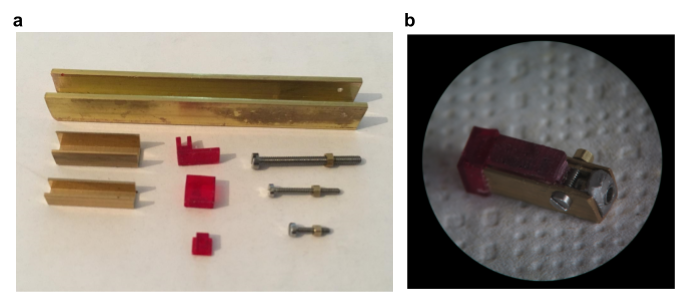
\includegraphics[width=150mm]{figures/F29_microdrive.png}}
\caption[Microdrive]{
Pictures of the custom-made microdrive. (a) 3D-printed and pre-cut brass parts, required to build the microdrive. (b) A picture of the assembled microdrive.
}
\label{fig:F29_microdrive}
\end{figure}

In the beginning of the project, I invested time to design the custom microdrive that meets these criteria (Figure 29 a and b). The major parts needed to assemble the microdrive are the U-shaped rails (commercially available), the M1 and M1.4 10mm screws (also commercially available) and the custom designed plastic parts. The Asiga Pico2 3D printer (https://www.asiga.com/) was used to print the plastic parts. The M1 driving screw having 250um height change per full turn allowed for the 31.25um single movement precision when rotated at 1/8 of a turn per adjustment. The total price of the required parts does not exceed 5 euros, the assemble time does not exceed 1 hour if the printed parts are ready. The drive was successfully implanted to 12 gerbils and proved it’s stability during the recordings. Most of the silicon probes were fully recovered after the end of the experiment, although some had to be trashed due to the surgical issues (recording shanks were clogged by cerebro-spinal fluid or some bleeding and the probe was not recoverable).

\subsection{Protecting box}

In contrast to the different designs of the tetrode drives, which are typically cemented to the skull together with the connector and protection for moving parts, the reusable microdrive with the recording device should be placed in a separate protective enclosure, disconnected from the drive itself. The standard procedure is to build this exclosure from copper mesh during the surgery, gradually building the shielding walls with cement. This method requires careful manipulation of the mesh parts with close proximity to the implanted probe and takes a long time, increasing the duration of the surgery and reducing the chances for successful recovery. The availability of high-precision 3D-printing in house allowed to design a custom protective box that can be assembled directly on the head of the animal during the surgery in a matter of a few minutes (figure 30a). The box has the following properties:

\begin{itemize}
    \item it is fast and easy to assemble during the surgery, easy to dismount at the end of the experiment
    \item it has a quickly removable cover for a) adjustments of electrode’s position, and b) changing the type of the cover from the simple protecting cover to the recording cover that has infra-red sensitive markers, required for tracking system
    \item it’s length and width do not exceed 18x18 mm to not interfere with gerbil eyes and ears position
    \item it is lighter than 3g to not exceed 5g of the total implant weight together with the microdrive
    \item it protects the recording device from dust (while animal is in cage) and light (during recording)
    \item it is strong and can last for long time (up to several months)
\end{itemize}

\begin{figure}
\captionsetup{format=plain}
\makebox[\textwidth]{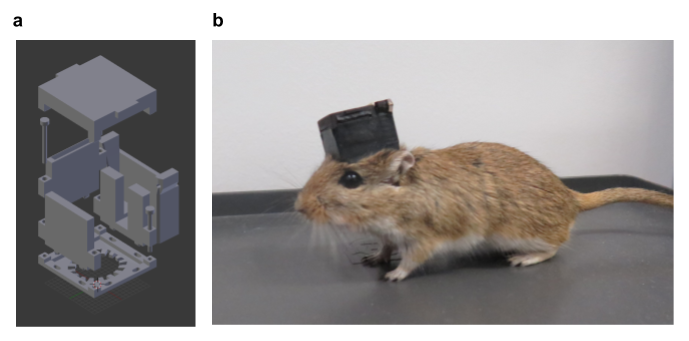
\includegraphics[width=150mm]{figures/F30_crown.png}}
\caption[Protecting box]{
(a) A 3D-model of the protecting box with the connector pocket. (b) A picture of the implant on the animal.
}
\label{fig:F30_crown}
\end{figure}

I designed the corresponding protecting box for 3D printing. I used 1x1.5x5 mm magnets, glued inside both the walls of the box and the top cover, to implement easy access inside for electrode adjustments. The M1 10mm screws were used to hold the walls together. As a result, the overall surgical time decreased and the new implant design allowed for the recovery of the recording device with the connector at the end of the experiment.

The designed protective box was successfully used in 12 animals (figure 30b), 4 of them for the duration of more than 2.5 months. Despite the light accumulation of dust inside the box, due to an imperfect connection between the top cover and the wall with the connector, the box was stable and reliable and didn’t show any failure in all of the animals.


\subsection{Surgery}

Standard stereotaxic surgical procedures of implantation of microelectrodes in the rodent hippocampal area CA1 were performed. Before the surgery, a 3D model prototyping the stages of the implantation was designed to ensure the correct placement of the microdrive and the protecting box, as well as the later fixation of the connector (figure 4.3 a-c). A 3-component solution with medetomidine-midazolam-fentanyl (0.15mg/kg, 7.5mg/kg, 0.03mg/kg) was used to anesthetize animals and keep the anesthesia for the duration of the surgery, by re-injecting the solution every 2 hours if the animal showed foot reflexes. During the surgery, animals were head-fixed in a stereotaxic frame (Stoelting Co.) placed on the heating pad with the termometer to maintain the body temperature of 36°C. All animals were implanted in the right hippocampus. A silicon probe oriented 15\% to the vertical plane attached to a microdrive was inserted into a 2mm wide craniotomy window (AP 3.0mm, ML 3.3mm, DV 0.9mm, averaged using the lambda-bregma distance according to the \cite{Radtke-Schuller2016}). Sealing wax was used to protect the electrodes and to cover the craniotomy window.

\begin{figure}
\captionsetup{format=plain}
\makebox[\textwidth]{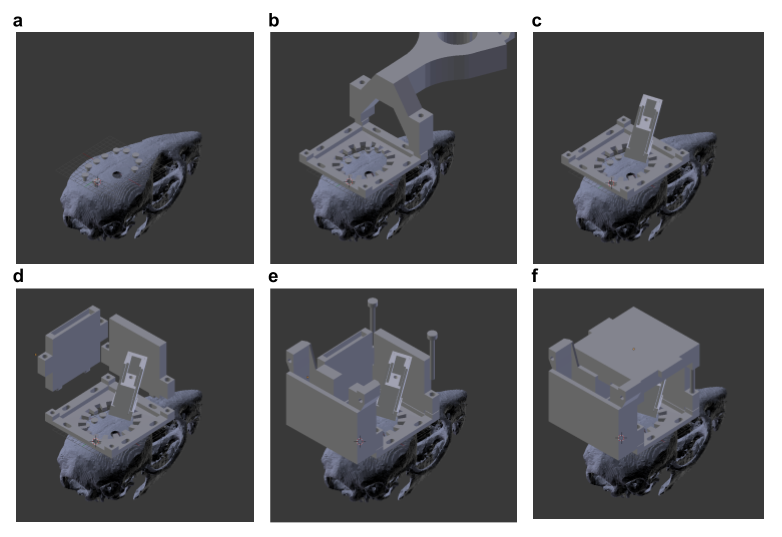
\includegraphics[width=150mm]{figures/F31_surgery.png}}
\caption[Surgical procedures]{
3D-modelled stages of the microdrive insertion and implant assembly during the surgery. (a) Insertion of the grounding screws to the skull. (b) Fixation of the base plate on top of the grounding screws. (c) Placement of the microdrive with the electrodes under the required angle and fixation of the drive with the cement. (d-e) Assembly of the protecting box using M1 10mm screws on top of the base plate. (f) The resulting implant assembled.
}
\label{fig:F31_surgery}
\end{figure}

The base plate, necessary to hold the protecting box, was cemented to the skull together with 10 M1 1mm screws, anchored to the frontal, left parietal and occipital bones (Dental cement, Paladur). Two screws inserted in the occipital bone above the cerebellum served as electrical ground. The surgery finished with the 3-component antagonist atipamezole-flumazenil-naloxone (0.4mg/kg, 0.4mg/kg, 0.5mg/kg). The post-surgical treatment included 5 days of daily injections of antibiotics (Baytril, 10mg/kg) and 3 days of analgesics (meloxicam, 0.2 mg/kg). The recordings started only after complete animal recovery.


\subsection{Recording procedures}

After the successful animal recovery the electrodes were adjusted daily to lower the probe tips with recording channels to the pyramidal layer of hippocampal CA1. Lowering of the electrodes was done in small increments of 1/8 to 1/4 of a turn (31.25 to 62.5um) not exceeding 125um per day to avoid damaging neural tissue and missing the right hippocampal layer. To make a proper adjustment, an animal was connected to the acquisition system before the move of the electrodes and the LFP signal was monitored. The correct placement of the electrodes was defined by several factors, including the presence of sharp waves (\cite{Buzsaki1986}) and ripples (\cite{OKeefe1978}) in the LFP signal during immobility periods, as well as the presence of simultaneous bursts of spikes pointing to the putative pyramidal cell activity in this region. If these factors were not observed within a reasonable time (approx. half an hour) the electrodes were adjusted and an animal was left for another half a day. Otherwise, an experimental session was recorded.


\subsection{Histology}

To confirm the correct electrodes location, a histology on the animal’s brain tissue was performed. Animals were deeply anesthetized with pentobarbital and perfused with 4\% paraformaldehyde. After the perfusion, brains were extracted and stored in paraformaldehyde for at least one day. Brains were sliced coronally in 60um slices and the slices near the craniotomy were stained with neutral red. Pictures of the slices were taken using the 10x microscope (see examples on figure 32).

\begin{figure}
\captionsetup{format=plain}
\makebox[\textwidth]{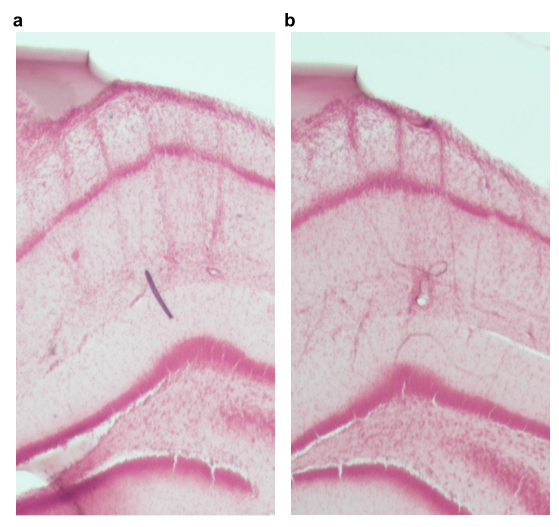
\includegraphics[width=100mm]{figures/F32_histology.png}}
\caption[Histology]{
Example pictures of histological slices. (a) Example picture from animal 00908 slide 6 slice 4 - 2x (b) Example picture from 003281 slide 6 slice 5 - 2x. Note multi-shank tracks of electrodes penetrating the CA1 pyramidal layer (top).
}
\label{fig:F32_histology}
\end{figure}


\section{Virtual reality setup}
\label{sec:vr_setup}

\subsection{RatCAVE system}

All experiments were designed to be conducted in a 3D virtual reality setup named ratCAVE (\cite{DelGrosso2018}). The setup consists of a large rectangular arena (floor area 162 cm × 72 cm and walls of 60 cm height, placed with a 70 degrees angle to accommodate the visual projection),a set of 7 infra-red tracking cameras (Prime 13W 240 fps, OptiTrack, NaturalPoint Inc., United States) located above the arena, and a high-frequency projector (Prime 13W 120 fps, OptiTrack, NaturalPoint Inc., United States), used to project a 3D virtual environment on the walls of the arena. Each experimental session a 3D-printed set of three spherical reflective markers was magnetically attached to the head of the animal, on top of the implant to not interfere with the headstage. These markers were tracked in a closed-loop by the cameras  to be able to adjust the projection depending on the animal's position. Blender (https://www.blender.org/) package was used to design the virtual environment and export it to .obj files, used by the custom-written 3D graphics python software (\cite{Grosso2019}) for rendering.

Two standard linear actuators and a bearing rail system were installed below the arena to physically move the arena ialong one coordinate axis. The maximum move was 30cm, limited by the borders of the projection. The actuators were controlled by an arduino with a motor shield, connected via USB / serial port to the computer with the experiment control software.

\begin{figure}
\captionsetup{format=plain}
\makebox[\textwidth]{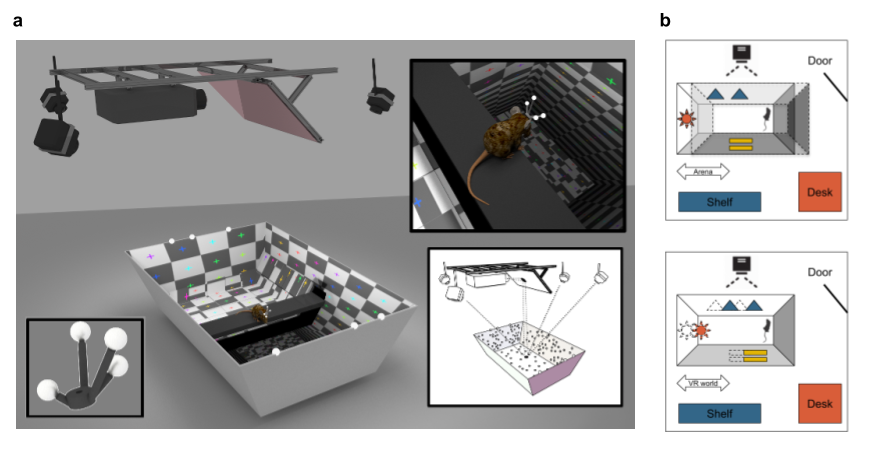
\includegraphics[width=150mm]{figures/F33_VR_setup.png}}
\caption[Virtual Reality Setup]{
The ratCAVE freely-moving virtual reality system for rodents used in experiments. (a) A 3D-model of the arena, position tracking and the projection systems. Left inset (left) shows the reflective markers placed on the animal's head, which is used by the tracking system to locate the animal (adapted from \cite{DelGrosso2018}). (b) Location of the arena in the experimental room and a schematic of the potential experiments: linear translation of the arena using linear actuators (top) or manipulation of the virtual projection (bottom).
}
\label{fig:F33_VR_setup}
\end{figure}


\subsection{Rewarding system}

A food dispenser (Campden Instruments Ltd.), positioned above the arena served for automatic reward administration. As most of the experiments were designed for random foraging, a food dispenser was triggered for dropping a food pellet (20 mg, TestDiet LabTab AIN-76A) at a random location within the arena at 1 minute intervals.


\subsection{Acquisition system}

An Open Ephys acquisition system (www.open-ephys.org , \cite{Siegle2017}) driven by an Opal Kelly XEM-6310 FPGA module was used to acquire neuronal data at a 30kHz sampling rate. The 32 or 64-channel Buzsaki H64 silicon probes were connected via the Intan RHD2000 series headstage to the acquisition box, which transmitted the raw data to the Open Ephys GUI for saving and visualization. The synchronization between the electrophysiology and virtual reality systems was done using the “Network Events” plugin, essentially implemented by periodic sending of TCP packets using python ZeroMQ package from the VR computer to the Open Ephys acquisition socket on the Ephys computer, connected directly via ethernet cable.


\subsection{Automatic experiment control}

A custom experimental control software was written to asynchronously manage the virtual projection, information from the tracking system, linear actuators, food dispenser, visualization of the animal position, video- and position logging and synchronization with the acquisition system. The non-blocking transmission of the information between components was implemented using the PUB/SUB communication scheme based on the ZeroMQ messaging system (https://zeromq.org/). Rendering of the virtual projection was performed by the ratCAVE package (\cite{Grosso2019}), food dispenser and linear actuators were connected and operated via USB serial ports, OpenCV (https://opencv.org/) was used for both video recording and animal position visualization, and built-in python components for metadata and logging.


\section{Data analysis}

Data analysis was primarily done in Python 3.5 with the standard math packages numpy and scipy, as well as scikit-learn, matplotlib and other utility packages. Partially the analysis was done in Matlab R2018b using standard libraries (detection of local minima, detection of center of mass of place fields). Significant amount of analysis was written in Jupyter notebooks for better visualisation. Analysis scripts, jupyter notebooks and the code implementing the data processing workflow are available in the project repository.


\subsection{Data processing workflow}

To increase efficiency and consistency working with large amounts of heterogeneous neuroscience data I developed a custom software automating the data processing workflow. A python package named “stapler” (https://gitlab.lrz.de/asobolev/stapler) was written to implement a pipeline consisting of the following steps:
\begin{itemize}
    \item collecting recording session data about animal positioning, animal electrophysiology and session configuration from the local PCs to the central storage
    \item merging corresponding data into a single folder
    \item converting OpenEphys files to binary formats, creating LFP files, compressing video files
    \item running spike sorting workflow on the raw data (high pass filtering, extracting spikes, PCA on spikes, running KlustaKwik, cleaning up)
    \item backing up unit clusters, syncing position and unit firing data, saving optimized data to HDF5
    \item performing post-processing steps required for final analysis (building place fields, calculate unit metrics, computing center of masses of place fields, running bootstrapping on the spiking data, running density based clustering, calculating place field shift matrixes, creating place field figures for every epoch)
\end{itemize}

The program allowed to change the running configuration for each step independently, enabling having custom processing parameters for different types of experimental sessions.


\subsection{Identification of single units}

Klusta (https://github.com/klusta-team/) software was used to perform spike clustering. The NeuroSuite (http://neurosuite.sourceforge.net/) was used to visualize raw data and to manually filter out noise clusters, as well as to merge similar clusters according to their burstiness and waveform shapes on corresponding channels. Clusters, representing interneurons by their spike width and average firing rate, were not taken into further analysis.
I used cluster isolation distance as a parameter to assess spike sorting quality (\cite{SCHMITZERTORBERT20051}). Clusters having isolation distance < 15 were excluded from further analysis.

\begin{figure}
\captionsetup{format=plain}
\makebox[\textwidth]{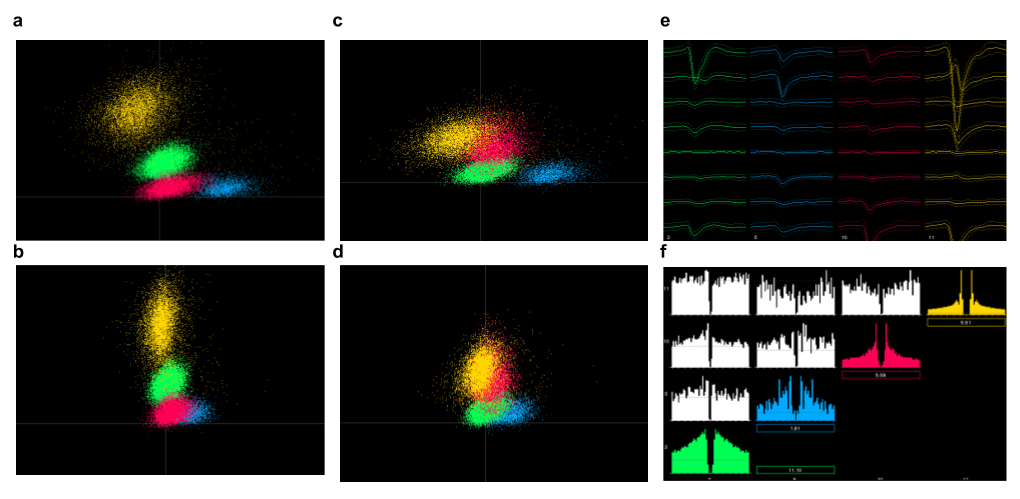
\includegraphics[width=150mm]{figures/F34_spikesorting.png}}
\caption[Spikesorting]{
Spike clustering. (a-d) Example cluster projections in pairs of principal components. Spike belonging to the same cell share the same color. (e) Example waveforms (mean) and (f) cross-correlograms of spiking of the same cells as in (a-d).
}
\label{fig:F34_spikesorting}
\end{figure}


\subsection{Spatial firing maps and place fields}

For every recording session and subsequent experimental condition I calculated spatial firing maps, mainly to visualize the conditional spatial selectivity - the change of the unit firing rate depending on the animal’s and arena position. The space was binned in 0.5 x 0.5 cm squares and the number of spikes for each bin was accumulated. The spiking map was computed by dividing the number of spikes in each square bin by the total time spent in the bin. The resulting firing rate maps were created by applying smoothing with 2D gaussian filter with sigma = 3 cm.

To define the precise analytical locations of place fields, I calculated the areas above the 0.5 * peak firing rate (threshold) of each firing rate map, and each connected area was taken as a putative place field. For each place field the center of mass (COM, Cx; Cy) was calculated:

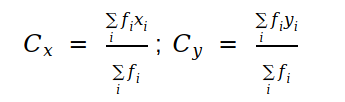
\includegraphics[width=70mm]{assets/formula.png}

where fi  is the firing rate and xi  yi  are the coordinates of the spatial bin. For each place field these centers of masses were not used as a final location of the field but used to further refine the position by bootstrapping.

To reach better precision on defining the place field locations, as well as to exclude noisy fields I used bootstrapping on the original spiking data. First, I split each spike train into several experimental conditions. For each condition I bin the timelapse of the spike train in chunks of 10-15 s and build a new spike train by randomly taking chunks with replacement. As a result of performing this operation 1000 times I get 1000 re-sampled place fields for each experimental condition. Second, for each new re-sampled spike train I compute individual place field locations using the thresholding / center-of-mass method, described above. This resulted in the number of bootstrapped locations of putative place field centers for each unit / condition. By design of the bootstrapping method, the centers of these individual fields tend to cluster together across all resamples if the field is stable, and tend to spread if the field is just noise. To get the actual fields, I used density-based spatial clustering with noise to separate well-connected clusters of bootstrapped field centers. The density-based clustering procedure allows to ignore noisy resamples (less than 100 field centers in the cluster from 1000 resamples), as well as to rank resulting clusters by the number of points (field centers) in the cluster. By taking the clusters with the highest rank I separate the most stable fields from the ones that hardly survive bootstrapping (practically I take the best 2 clusters, e.g taking 2 fields per unit maximum). Finally, the center of each cluster given by the density-based clustering was taken as a final place field location (figure 34 a-c).

\begin{figure}
\captionsetup{format=plain}
\makebox[\textwidth]{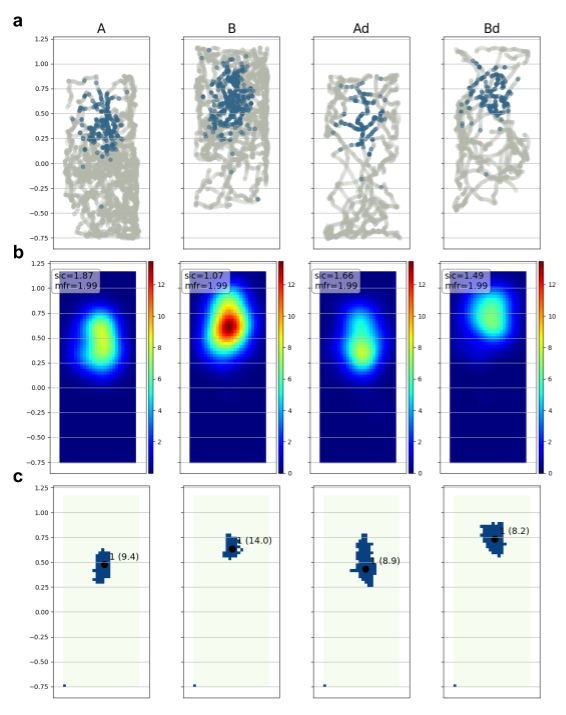
\includegraphics[width=100mm]{figures/F35_place_fields.png}}
\caption[Place field detection]{
Detection of place fields. (a) Example spiking (blue) and arena occupancy (grey) plotted in the arena coordinates. (b) Example firing rate maps of a neuron in (a). (c) Place field patches and their center-of-masses computed using the bootstrapped procedure
}
\label{fig:F35_place_fields}
\end{figure}


\subsection{Place field shift detection}

For each cluster I use it's surface projection to calculate corresponding fields between experimental conditions (Figure 35c). By gradually shifting one projection relative to another in a range from 0 to 0.3 m (the shift of the arena or the virtual projection in all experiments) and computing the maximum of their overlap I determined the clusters which projections overlap the most (if a field in A does not overlap with any other field in B it means it remapped). After the fields are "paired" between conditions the vertical difference between the centers of their clusters (literally center-of-mass of their bootstrapped field centers) is computed as a shift of that particular field between given conditions (Figure 36).

\begin{figure}
\captionsetup{format=plain}
\makebox[\textwidth]{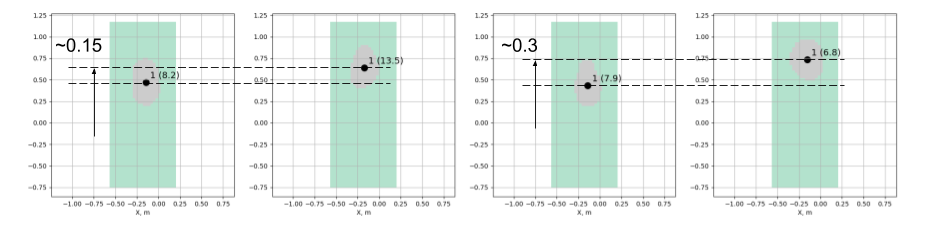
\includegraphics[width=150mm]{figures/F36_shift_detection.png}}
\caption[Field shift detection]{
Detecting place field shift. An example place field with patches in all experimental conditions. This example has only one place field, it has a shift along the Y-axis of 0.15m (light condition, left two plots) and a shift of 0.3m (dark, right two plots).
}
\label{fig:F36_shift_detection}
\end{figure}
